%Settings{{{
\documentclass[12pt]{iopart}
\usepackage{graphicx}
\usepackage{iopams}

% Fixing iopams poor centering of equations:
\expandafter\let\csname equation*\endcsname\relax
\expandafter\let\csname endequation*\endcsname\relax
\usepackage{amsmath}
%
%}}}

%Plan {{{ 
% Title
%% Make sure that I only talk about areas I am really interested in and want to talk about. 


%% State of the art experimental apparatus for fast entangling gates in trapped multi-ion crystals

%% 11 Page limit

%% (Short) intro to trapped ion QC and Theory on Fast Gates schemes: ~ 2 pages

%%     * Motivating why QC important. ~ 1 paragraph

%%     * Trapped Ion QC - General idea of spin (ion) coupled with HO (Trapping potential) and how this satisfies QC requirements. ~ 1-2 paragraph

%%     * Entangling gates MS gate. Statement of Hamiltonian and how this is experimentally realised. ~ 1 paragraph

%%     * Fast Gate Schemes (Non-Adiabatic Entanglement). Amplitude shaped pulses. ~ 1 sentence and reference
%%         Why we want to move to quadrupole optical transition rather than Raman (Scattering error and squeezing term)

%%     * Carrier Nulling. (excerpt from paper starts) ~ 2 paragraphs

 

%% Experimental results from Carrier Nulling (excerpts from paper): ~ 2+ pages

%%     * Description of Blade ~ 1 figure + 1 paragraph

%%     * Phase control ~ 1 paragraph

%%     * Proof of principle on Blade apparatus ~ 2 paragraph (statement of results) 2 figures

%%     RBM work ~ few sentences

 

%% FastGates buildup: ~ 4 pages

%%     * Motivation for why we want a new system (compare with Blade) ~ 1 paragraph

%%     * Description of FastGates – central figure of full physical experiment and figure of control systems ~ 2 paragraphs large figure
%%         In effect list all the benefits over Blade - and how it fits into requirements for NISQ?

%%     Now looking at components of new system from center outward:

%%     * Ca40 energy diagram  ~ 1 paragraph and energy level figure
%%         Simple energy structure. Less spectator modes compared to Ca43 -> less off resonant transitions. But sensitive to B field.

%%     * NPL trap, trap frequencies, substrate bias for crystal rotation ~ 1 paragraph 1 figure
%%         What trap freq do we want for fast gates 

%%     * In vacuum system details ~ 1 paragraph 1 figure

%%     * Dual Optical Access High NA system ~ few sentences

%%     * Single Ion Addressing with AOD, power requirements ~ 1 paragraph
%%         This is potentially a drain of time – time bound looking into this.

%%     * Addressing and Readout optics design? ~ short 1 figure

%%     * Extension to standing wave single ion addressing – ideas/design for phase feedback ~ few sentences 1 figure?

%%     * 729 system design, PDH locking, FNC ~ 1 paragraph

   

%% Outlook: ~ 1 page

%%     * Overall goals of project
%%         - Optical phase control of laser field at the ion.
%%         - Fastgates on multi ion chain.

%%     * Immediate tasks: Finishing vacuum work, trap on table. Trapping ions 

%%     * Proposed first experiments? 
%%         1st paper: EOM to keep stark shift the same as pulse amplitude changes 
%%         Explore this for 1 day
%%             Ask about scheme 
%%             This is a problem with gates with multiple pulses. 
%%                 Theory on this

%% What will my next 6 months, 1 yr, 2 yrs look like? 
%}}}

%Opening{{{
\begin{document}
\title[]{State of the art experimental apparatus for fast entangling gates in trapped multi-ion crystals}

\author{Donovan Webb}

\address{Department of Physics,
University of Oxford}
\ead{donovan.webb@physics.ox.ac.uk}

\begin{abstract}

    Scalable trapped-ion quantum computation relies on the development
    of high-fidelity fast entangling gates in many ion crystals.
    %
    Currently the speed of geometric phase gates are limited by either large
    scattering errors (with Raman transitions) or off-resonant carrier
    excitations (with quadrupole transitions).
    %
    Utilizing standing waves offers a potential pathway to achieve
    fast entanglement in quadrupole transitions due to suppressing
    undesired carrier excitations.
    %
    Using a legacy apparatus we present initial results of this
    carrier suppression in the~$674$~nm quadropole transition of
    \textsuperscript{88}Sr\textsuperscript{+}. We demonstrate
    fast two-qubit entangling gates which exceed the entangling ``speed
    limit'' imposed by off resonant carrier excitations.
    %
    To explore these ``fast gates'' at durations comparable to the
    secular trap frequency, and in multi-ion chains, a new system is
    been constructed. This system will use a segmented 3D Paul trap
    for greater control of long ion chains, and will feature single
    ion addressing for both selective and high power coherent
    operations.  We present the current progress and roadmap of this
    next-generation platform and motivations behind design choices.

\end{abstract}
%}}}

%Introduction {{{
\section{Introduction}

    *Trapped Ion QC\\
    General idea of spin coupled with HO\\
    *Entangling gates MS gate \\
    *Non-Adiabatic interactions \\
    *Fast Gate Schemes \\

Previously the physicist was limited to thought experiments on the
Quantum nature of single particles. It was inconceivable to isolate,
probe and entangle together single particles. However the advent of
Ion traps, specifically Paul and Penning traps, have enabled the
experimental exploration and corroboration of Atomic theory producing
incredibly precise measurements such as XXclocks, relativity, g
factorXX [clocks, relativity, g factor].

With the high degree of experimental control of a quantum system
exhiibited by Ion trap systems, they are an obvious and increasingly
mature platform for enabling Quantum Computation.

Ion-traps trap ions through a combination of static and oscillating
electric fields. Ions will sit at local minima of this potential and
experience harmonic motion. When $N$ ions are trapped
simultaneously they may form linear strings or crystals due to the
combination of trapping potential and mutual repulsion between
like charged ions. A linear crystal of N ions will exhibit $3N$ normal
modes. These single ions within the crystal may be modelled as two
level ``spin'' systems, whilst the harmonic motion is modelled as a
``spring'' system. We may utilize the shared motion of ions to
entangle their spin states.

Describe entangling...
With Lamb-Dicke approximation:
H = Carrier + eta*SB


    Controlled light-matter interactions are essential for quantum
    computing [1–3], quantum simulation [4, 5], and metrology [6,
      7]\\

    ******************  From paper  ************************\\
    For trapped ions, controlled light-matter interactions typically require
    carrier interactions that only couple the internal qubit states,
    as well as sideband interactions that couple these internal states
    to their collective motion [3]. For example, the sideband
    interactions, driven by the spatial gradient of the carrier
    coupling, are used to mediate spin-spin interactions such as
    entangling gates [8]. Conventionally, coherent control of
    laser-ion interactions is achieved using traveling waves (TWs)
    [3]. As the ions experience an averaged electric field and
    gradient over the interaction duration, the ratio between carrier
    coupling and sideband coupling is fixed. In contrast, the coupling
    strengths for ions in a standing wave (SW) vary with the spatial
    structure of the light field along the propagation
    direction. Consequently, the phase of the SW at the ions sets the
    ratio between the carrier and the sideband coupling. Coherent SW
    interactions on a single ion have been studied previously using
    cavities [9, 10], integrated optics [11] and free-space approaches
    [12]. However, coherent operations on multiple ions with a SW have
    so far been unexplored.\\

    The tunability of the carrier:sideband coupling ratio is especially
    important for strong interactions where off-resonant terms start
    participating significantly and cannot be eliminated
    adiabatically. For example, in the conventional Mølmer Sørensen (MS)
    mechanism [13], the TW that generates the spin-motion coupling also
    gives rise to an off-resonant carrier coupling, which causes an error
    in the entangling operation. This error becomes significant as the
    carrier interaction strength approaches the motional frequency,
    placing a limit on the speed of the entangling operation. Using a SW
    instead enables high-fidelity entangling operations that can surpass
    this speed limit by selectively enhancing the spin-motion coupling
    while coherently suppressing the detrimental carrier term [14].\\


    We show that the
    presence of the carrier coupling term, in the context of the TW-MS
    gate, leads to a reduction in the spin-dependent force (SDF)
    magnitude, which scales with the Rabi frequency of this detrimental
    term, posing an inherent speed limit for this mechanism.

    It can be shown that a travelling wave MS in the interaction picture obeys
    equation 4 of paper, where the SDF follows a bessel like
    relationship as shown in fig X, featuring a global maximum
    achievable force amplitude. This maximum point direclty limits the
    speed at which gates can be achieved.\\
    ***********************************************************\\
%}}}

%Results and Discussion {{{
\section{Carrier Nulling Results}

    Excerpts from carrier nulling paper kind of want to put this after the FG description... Or could I shorten this massively to reduce emphasis?\\
    
    As discussed in sectionXX, the use of phase-stable standing waves (SW) is a clear route to fast entangling gates on quadrupole transition qubits. 
    Here we report experimental results of both SW single qubit gates and SW Molmer Sorensen (MS) entangling gates performed on the Blade apparatus.\\

    We use a free-space, phase-stabilized SW formed by two
    superimposed counter-propagating 674-nm beams that couple to the
    quadrupole qubit transition, 5S1/2 ↔ 4D5/2, in 88Sr+.\\

    **Here quadrupole so gradient couples carrier whilst XXCurlXX couples the sideband interaction\\.

    The single-qubit gate is created using a monochromatic SW on
    resonance with the qubit transition while placing the node(s) of
    the SW at the position of the ion(s). The two-qubit entangling gate
    is implemented via an MS-type scheme where we use a bichromatic SW
    instead of the conventional bichromatic TW.\\

    Using the
    SW-MS instead, with the anti-nodes placed at the ions, we strongly
    suppress the undesired carrier term and show that we can surpass
    this speed limit.\\

    %% ******************* Appendix? ****************
    %% * Could shift these derivations to the intro. \\
    %% First derivation of equation 1 of paper. \\
    %% By setting δ = 0 or δ = ±ωz, we can bring the carrier or sidebands
    %% into resonance, respectively. With ∆φ the SW has an additional
    %% degree of freedom compared to the TW: by setting 2 ∆φ = 0 we can
    %% drive the first sidebands while suppressing all even terms in the
    %% Lamb-Dicke expansion [26], including the carrier term. Conversely,
    %% if we set ∆φ = π we drive the carrier coupling and suppress all
    %% odd terms in the Lamb-Dicke expansion, including the first
    %% sidebands. \\

    %% The MS interaction requires two tones symmetrically detuned about the
    %% qubit resonance by δ ≈ ±ωz. To construct the Hamiltonian for a SW-MS
    %% interaction, we combine two monochromatic SWs as described by Eq. (1),
    %% resulting in the bichromatic SW interaction\\
    %% Equation 2 from paper\\

    %% where the phase ̃ φ =( ̃ φBD + ̃ φRD)/2 is now the mean optical phase
    %% between the blue- (BD) and the red- (RD) detuned SWs. Further, we
    %% assume that the BD and RD SWs are in phase at the position of the
    %% ion(s), i.e. ∆φBD = ∆φRD = ∆φ . The first term corresponds to a
    %% spin-dependent force (SDF) and the second term drives the carrier
    %% transition off-resonantly. Notably, these terms commute. Similar to
    %% the monochromatic SW, we can drive the motional coupling while
    %% suppressing the spurious carrier coupling by setting ∆φ = 0.\\

    %% ***********************************************

    **Look at poster for description of phase feedback onto the ion -
    maybe exclude this to shorten section.\\

    still to tidy Results: \\
    We probe the position of the SW relative to a single ion by applying a
    monochromatic SW pulse on resonance with the qubit transition
    [Figs. 1(b), 2(a)]. The pulse duration corresponds to a π-pulse at
    maximum carrier coupling, which occurs at the nodes of the SW. For an
    electric quadrupole transition, the maximum carrier coupling occurs at
    the maximum gradient of the electric field [9]. We can maximize the
    carrier coupling and minimize the sideband coupling, or vice versa, by
    selecting ∆φ = π or ∆φ = 0 [Fig. 2(b)]. The transfer probability shown
    in Fig. 2(a) has a quartic dependence on ∆φ near ∆φ = π and a
    quadratic dependence at ∆φ = 0 [26]. When probing the suppressed
    motional sideband [Fig. 2(b) left], we observe only features that are
    due to the off-resonant (by ≈ 1.2 MHz) carrier coupling. By changing
    ∆φ of the SW, we can realise any ratio between carrier and sideband
    coupling.\\


    %% We measure Rabi frequencies by scanning the SW pulse
    %% duration at the carrier resonance, for both ∆φ = π and ∆φ = 0. We
    %% observe this ratio to be 18, corresponding to a suppression 01234 2Ω/δ
    %% 0 20 40 60 80 Ω /2π (kHz) SDF traveling wave standing wave 024 2Ω/δ
    %% 0.0 0.5 1.0 Ω /(ηΩ) SDF FIG. 3. Spin-dependent force magnitude ΩSDF
    %% (normalized by ηΩ in the inset) versus 2Ω/δ , as measured for a single
    %% ion with η = 0.05. We extract ΩSDF by applying a conventional
    %% bichromatic TW field (squares) or a bichromatic SW field (triangles),
    %% for variable durations. The solid lines show the analytical
    %% dependence; as predicted by the theory and shown explicitly in the
    %% inset, the TW coupling follows the Bessel functions (|J0 + J2|), while
    %% the SW coupling remains constant [34]. of 25 dB between maximal and
    %% minimal carrier coupling. This suppression is consistent with the
    %% measured interferometric stability and the residual power imbalance
    %% between b1 and b2.\\

    Expand this section and show some data of RBM results:\\
    Furthermore, we perform randomized benchmarking [32] to evaluate
    the quality of single-qubit gates implemented using the SW and TW
    with the same duty cycle. We obtain an error of 1.44(3) × 10−3 and
    1.73(3) × 10−3 per Clifford gate, respectively. Thus, use of the
    SW is not detrimental to single-qubit control. \\

    %% This has a lot of experimental detail. Maybe too much for the report.\\
    %% Next, we experimentally investigate the saturation effect caused
    %% by the non-commuting carrier coupling [Eq. (3)] when generating an
    %% SDF with a bichromatic TW, and compare it to the SDF generated by
    %% a bichromatic SW. To create the TW bichromatic field, we apply two
    %% tones to the AOM in b1, while for the SW we apply the same two
    %% tones in both beams, b1 and b2. These tones are symmetrically
    %% detuned by δ ≈ ±ωz from the qubit resonance. This results in an
    %% SDF on the axial mode (ωz/2π ≈ 1.2 MHz) of a single ion. We
    %% extract its coupling strength ΩSDF(Ω, δ ) by applying the SDF for
    %% variable durations [29]. We used an adiabatic ramp duration of 3.6
    %% μs for these measurements [33]. For the TW, we observe a coupling
    %% that scales with the expected Bessel function dependence |J0(2Ω/δ
    %% ) + J2(2Ω/δ )| [Eq. (4), Fig. 3]. Hence, when using the TW, there
    %% exists a maximum achievable interaction strength that imposes a
    %% speed limit on the interaction regardless of the available laser
    %% power. This limit is caused by the increasingly strong offresonant
    %% non-commuting carrier excitation and not by technical aspects such
    %% as pulse shaping. For the SW, we demonstrate that no such
    %% speed-limit exists. We place the ion at the maximum intensity of
    %% both the red- and the blue-detuned SWs [26] and observe that the
    %% interaction magnitude [34] increases linearly with Ω (Fig. 3).\\

    We experimentally demonstrate two-qubit MS gates using a bichromatic
    TW for gate speeds in a regime where the carrier coupling induces a
    significant error which cannot be eliminated adiabatically. However,
    the bichromatic SW enables us to surpass this limit without degrading
    the fidelity (Fig. 4). To implement the SW-MS gate, we simultaneously
    suppress the carrier coupling on both ions by adjusting the ion
    spacing such that they are both placed at anti-nodes of the SW
    [Fig. 1(c)] [26]. We perform the TW and SW two-qubit entangling gates
    on the axial in-phase mode and optimize the experimental parameters to
    maximize the Bell-state fidelity for a fixed gate duration. In both
    cases, we use a ramp duration of 10 μs to minimize coupling to the
    other motional modes [33]. This pulse ramping could be replaced with
    more sophisticated amplitude shaping techniques [16, 35]. In Fig. 4(a)
    we show the two-qubit fidelities achieved with the two schemes as a
    function of the effective gate duration (2π/δg, where δg = δ − ωz)
    [37]. For slower gates, the fidelity of the SW-MS is comparable with
    that of the TW-MS. For faster entangling gates, the fidelity of the
    TW-MS degrades rapidly. This is also predicted by direct numerical
    integration of Eq. (3); we set all the parameters to the experimental
    values except for the Rabi frequency Ω, which we optimize for maximum
    fidelity (dashed line). We also indicate the idealized case which
    neglects imperfect transfer into the interaction picture w.r.t. the
    carrier [Eq. (3)] (dotted line). We believe that the measured
    fidelities degrade sooner as a result of experimental imperfections
    (e.g. ramp shape) not captured by the numerical integration. In
    contrast, the fidelity for the SW-MS is consistent with ≈ 0.95 over
    the entire available power range, showing that we have eliminated the
    limit arising from the carrier coupling. The shortest SW-MS gate was
    15 μs, limited by the available total power of 29 mW. \\

    *Shorten conclusion and change in such a way that focusses on what to
    improve/adapt in FG setup\\

    In conclusion, we implemented single- and two-qubit operations for
    trapped-ion qubits using a phase-stabilized SW. Two
    counter-propagating beams create the SW, whose relative phase ∆φ at
    the ion position is stable to ≈ λ /100. This enabled us to tune the
    ratio of the field intensity and gradient that the ions experience,
    which sets the relative strengths of the sideband and carrier
    interactions. We use this new degree of control to suppress the
    unwanted off-resonant carrier coupling (by a factor of 18), while
    coherently enhancing the motional coupling during two-qubit gates. We
    show theoretically and experimentally that the non-commuting carrier
    term imposes a limit on the speed of conventional TW-MS gates, which
    were avoided using the SW-MS interaction. These optical phase control
    techniques could also be applied in the previous Raman-based scheme
    [16], where they could mitigate squeezing terms, which were the
    leading error source; we note that for the SW-MS those terms are
    inherently suppressed. Our work shows a clear path towards entangling
    gates with durations comparable to the motional period of the ions (∼
    1 μs or shorter) at wavelengths that are amenable to largescale chip
    integration using standard integrated optics [3840] and without the
    technical challenges of using high-power blue Raman beams [16], pulsed
    lasers [41, 42] or Rydberg schemes [43].\\

    - The ability for single addressing allows MS gate between two ions in a multi ion chain.\\
    - Also higher intensity at ion can push quadrupole gate time down to speeds where other motional mode inclusion matters (vera).\\
    - Hence explore Fast Optical transition gates at 729 nm in multi ion chain.\\
    
%}}}

%Experimental Details {{{
\section{Experimental Details}

The technical complexity of ion trapping experiments may be reduced to
solving two problems: Controlling the state of the ion (both internal
and motional); and controlling the environment the ion is within.
Our Ion trap experiments consist of: an atomic source, a trap, a
vacuum system encasing these, external magnetic field coils, and
lasers for ionization, cooling, repumping, stateprep, coherent
control and readout.
As with all ventures in experimental physics, as technologies mature, so
too do the capabilities and scope of our apparatus.  Here we shall
describe both the ``old'' apparatus, known in short as ``Blade'', where
proof of principle fast gate schemes have been tested, and the new
proposed system, known as ``FastGates'', which solves critical
limitations of ``Blade'' for further exploring fast entanglement and
non-adiabatic interactions.

\subsection{Ion and Trap}

\begin{figure}
  \begin{center}
   \noindent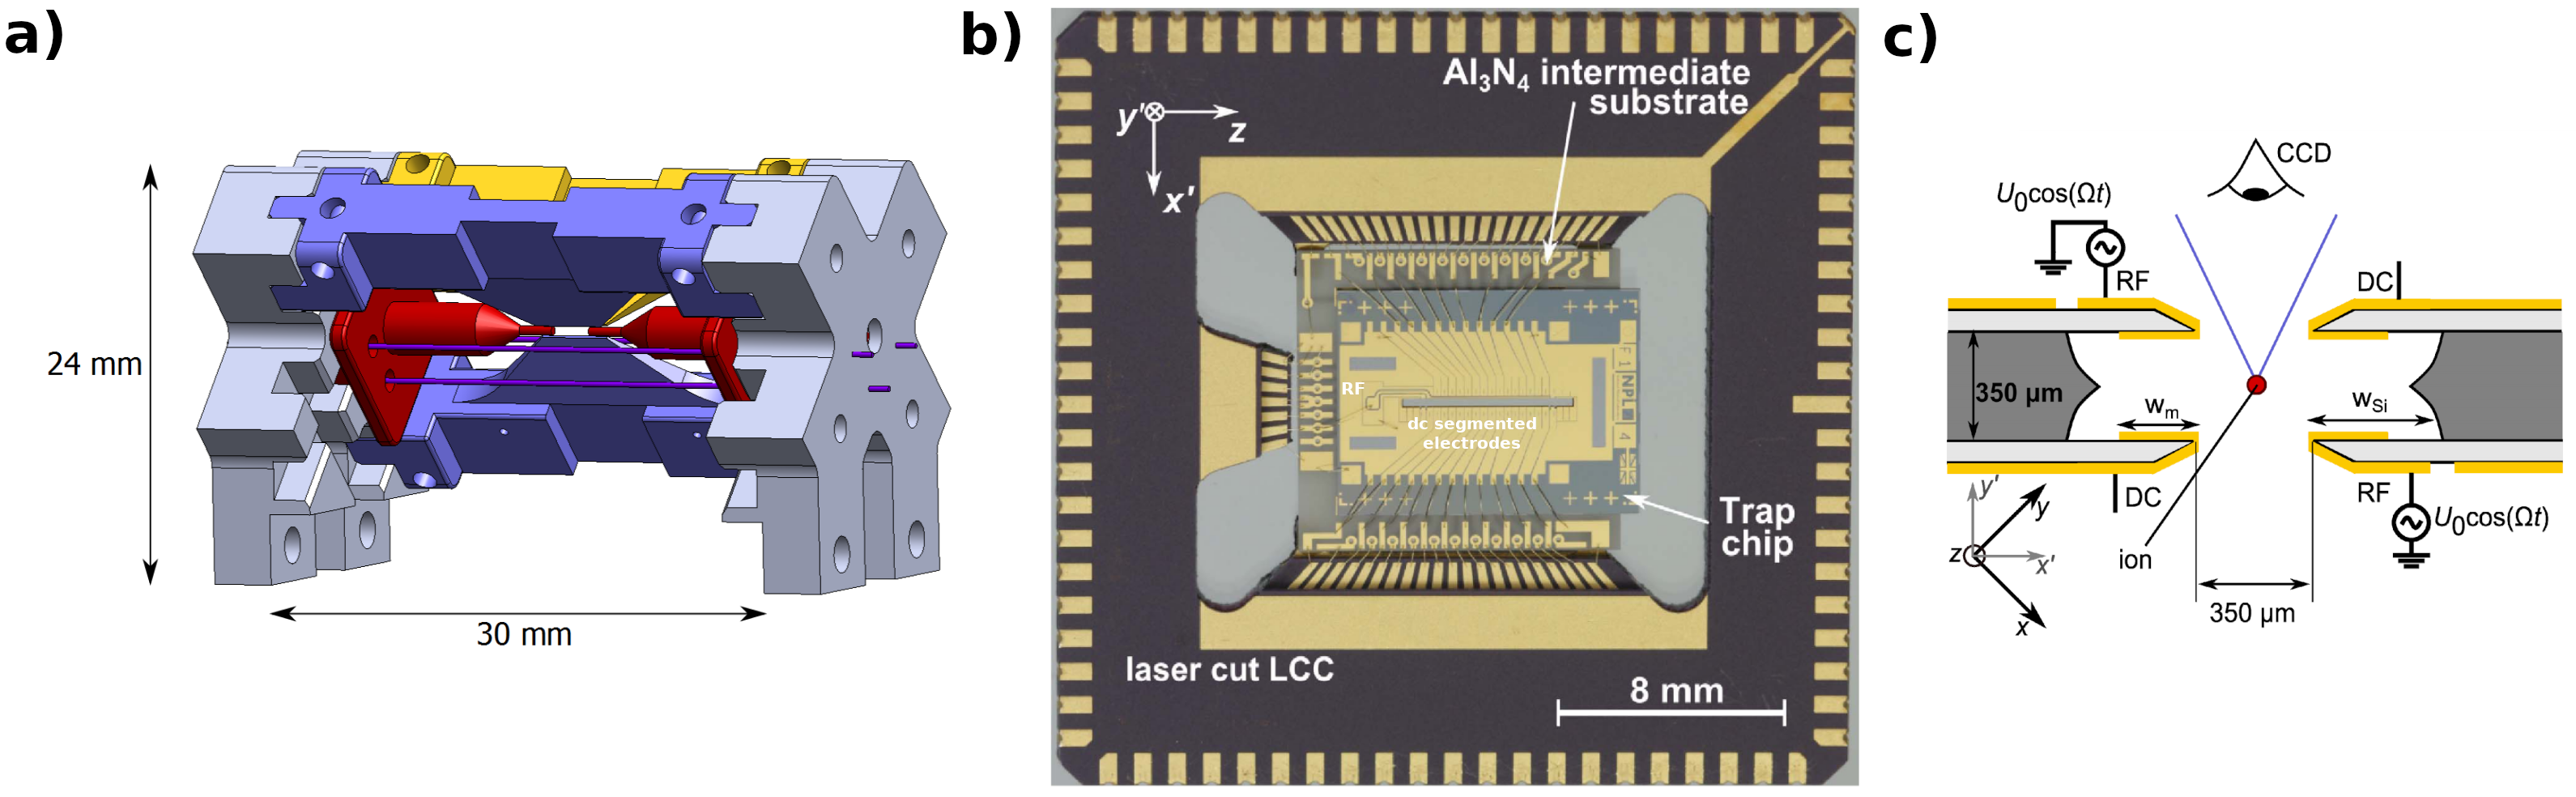
\includegraphics[width=\linewidth]{figures/trap_comp.png}
  \end{center}
  \caption{Blade and NPL trap
  figs from S. R. Woodrow. Linear Paul trap design for high-fidelity ,
  scalable quantum information processing. Master’s thesis, University
  of Oxford, 2015 and [1] K. Choonee, G. Wilpers, and A. G. Sinclair,
  ‘Silicon microfabricated linear segmented ion traps for quantum
  technologies’, in 2017 19th International Conference on Solid-State
  Sensors, Actuators and Microsystems (TRANSDUCERS), Jun. 2017,
  pp. 615–618. doi: 10.1109/TRANSDUCERS.2017.7994124.}

  \label{fig:trap}
\end{figure}

XX Table comparing appropriate dims/freqs/pots of three traps XX\\

As mentioned, the overall system we desire is a spin coupled to a
spring. Our spin in this case being a Hydrogen-like ion, and the
spring being the harmonic motion of the ions within the trapping
potential. The ion traps we use to create such a potential are linear
Paul traps, a schematic of such is shown in FigureX. As explained by
Earnshaw's theorem, $(\nabla^2 V = 0),$
a stable stationary point in 3D can not be realized using a static
electric potential, $V$, as if the potential is confining in 2
dimensions, it will be anticonfining in the third. Therefore to
achieve stable trapping a psuedopotential must be utilized.
%Include pseudopot eqn?
A Paul trap achieves this through an oscillating electric field
providing radial confinement and a static field to create axial
confinement. There are various popular geometries for realizing a Paul
trap: Macro 3D Blade traps; surface traps; and microfabricated
segmented 3D traps.  A Blade trap, as is used in the ``Blade''
apparatus, has axial confinement created by DC end caps and radial
confinement by supplying an oscillating RF voltage to the blades. In
``Blade'' the ion endcap distance is $1.15$~mm, and ion-blade distance
is $0.5$~mm. Typical operating frequency for the RF electrodes of the
``Blade'' trap are $28.0133$ MHz leading to an axial ion frequency of
$1.860$ MHz and radial frequencies of $4.077$ MHz and $4.341$ MHz.

Recently the surface style linear Paul
trap has gained popularity due to the maturity of chip fabrication
technologies and the potential route to scalability this offers. In
the surface trap, the 3D blade and endcap geometry of the ``macro''
trap is effectively projected onto a 2D surface. The stable point of
such a trap is typically on the order of $50$ um from the chip
surface. The ease of fabrication of surface traps has allowed the
creation of complicated multizone devices with many DC electrodes.
These multizone traps enable the shuttling of ions, a requirement for
Quantum CCD type architectures. However these benefits come at the
cost of trapping potential. Heating of an ion is XXproportionalXX to
the ion electrode distance, however so too is the trapping
potential. This leads to a compromise of distance... surface trap
creates a poor approx of harmonic potential... Therefore weak trap and
high heating rates compared to a macro 3D blade trap. Heating rates of
HOA2: axial and radial frequencies...

A microfab 3D trap [See et al and Wilpers 2012], as will be used in
the ``FastGates'' apparatus, brings together the advantages of chip
fabrication as well as the low heating rates and high trapping fields
of a 3D style trap. This is achieved by a multilayer chip as shown in
figureX. The radial trapping is provided by RF rails on opposite
diagonals of the slit whilst axial trapping may be realized by DC
electrodes on both surfaces. The Ion electrode distance is now of the
order $200$ um, meaning lower heating, whilst the more optimal 3D
geometry allows for a deep potential at this distance (XX 50x surface trap [Guido]). The
microfabrication techniques also allow a segmented design suitable for
multizone operations and ion shuttling.  The 3D confining potential
leads to motion of the ions following the Hamiltonian

$$ H = \sum_{i=1}^N \frac{m}{2}(w_x^2x_i^2 + w_y^2y_i^2 + w_z^2z_i^2 + \frac{|p_i|^2}{m^2}) + \sum_{i=1}^N\sum_{j>i}\frac{e^2}{4\pi\epsilon_0|r_i - r_j|}$$,

where $w_v$ are the mode frequencies in the three dimensional
coordinated. We define $z$ to be the axial direction of the trap and
typically assume $w_z$ << $w_x$, $w_y$ to allow a 1D ion crystal to
lie along the axial direction of the trap. We aim for an axial ion
separation of around $5$~um which, for $^+Ca_{40}$ ions means a
trapping potential of $w_z \approx 2\pi * 1.6$~MHz. This ion
separation was chosen to reduce the cross talk between ions when
singly addressed (see section X). We plan for around $5$~MHz for our
radial frequencies as we will use one such mode for implementing
two-qubit entangling gates. This higher frequency is for a few
reasons. Firstly, the doppler cooling limit
($\overline{n} = \Gamma/w$, where $\Gamma$ is the transition linewidth
and $w$ is the frequency of the mode being cooled) goes with the
reciprocal of the mode frequency and so higher mode frequencies leads
to a lower temperature after cooling. Secondly, a higher c.o.m. radial
mode leads to better separation of radial modes in a multi-ion crystal
which, if we implement the amplitude pulse shaped fast gate scheme
described above, can lead to pulse solutions with fewer segments. XX
Thirdly, can push to faster gates?

The radial mode frequency is given by
$w_{rad}$ equation. \\
Simulations of the NPL trap,
we require an $\Omega_{RF} = XX20$~MHz with a driving amplitude of
$180$~V to find a solution with axial frequency of 1.6MHz and a radial
frequency $w_x = 5$~MHz.

One foreseeable issue with this arrangement becomes apparant when
considering the Matthiu equation representing trapping with
pseudo-potential. There are areas of stability and instability which
can be quantified with the factor $q$. In Ion traps it has been shown
that areas of stability exist for $q<0.9$, however typical values of
$q$ for trapping and cooling ions are considerably smaller.
$q = 2*\sqrt{2}w_{ax}/\Omega_{RF}$.
For the proposed plan of $20$~MHz RF and $5$~MHz radial frequency we
would have $q = 0.7$ which although is still stable, may not be able
to practically trap from a hot source of ions. Therefore we will
likely trap at a lower RF amplitude, lowering the radial frequencies
to around $2$~MHz where $q<0.3$ and then ramp up to a tighter trap for
efficient doppler cooling and fast gate experiments.

Some simulations to find solutions with decent axial and radial modes and figures.

Heating rates... Further, the ion being located within this
slit allows for dual high NA optical access (NA = XX), which is an
important factor for our proposed single addressing standing wave
experiment.

\subsection{Laser systems}

We have described the trapping of an ion, now we must look at our
strategies for manipulating the internal states and collective motion
of ion strings. Lasers are a key tool for this as highly localised,
strong electric fields amplitudes and gradients can be produced.

First let us consider the \textsuperscript{40}Ca\textsuperscript{+} energy
level structure, figure X. The \textsuperscript{40}Ca\textsuperscript{+} has
no nuclear spin and is hydrogen like with only one external electron
giving a (relatively) simple level structure. An external magnetic
field of $5$ G is applied to Zeeman split the levels. The relevant
laser transitions for our planned ion trap experiment have been marked
and their purpose and construction shall be discussed below.\\

\begin{figure}
  \begin{center}
   \noindent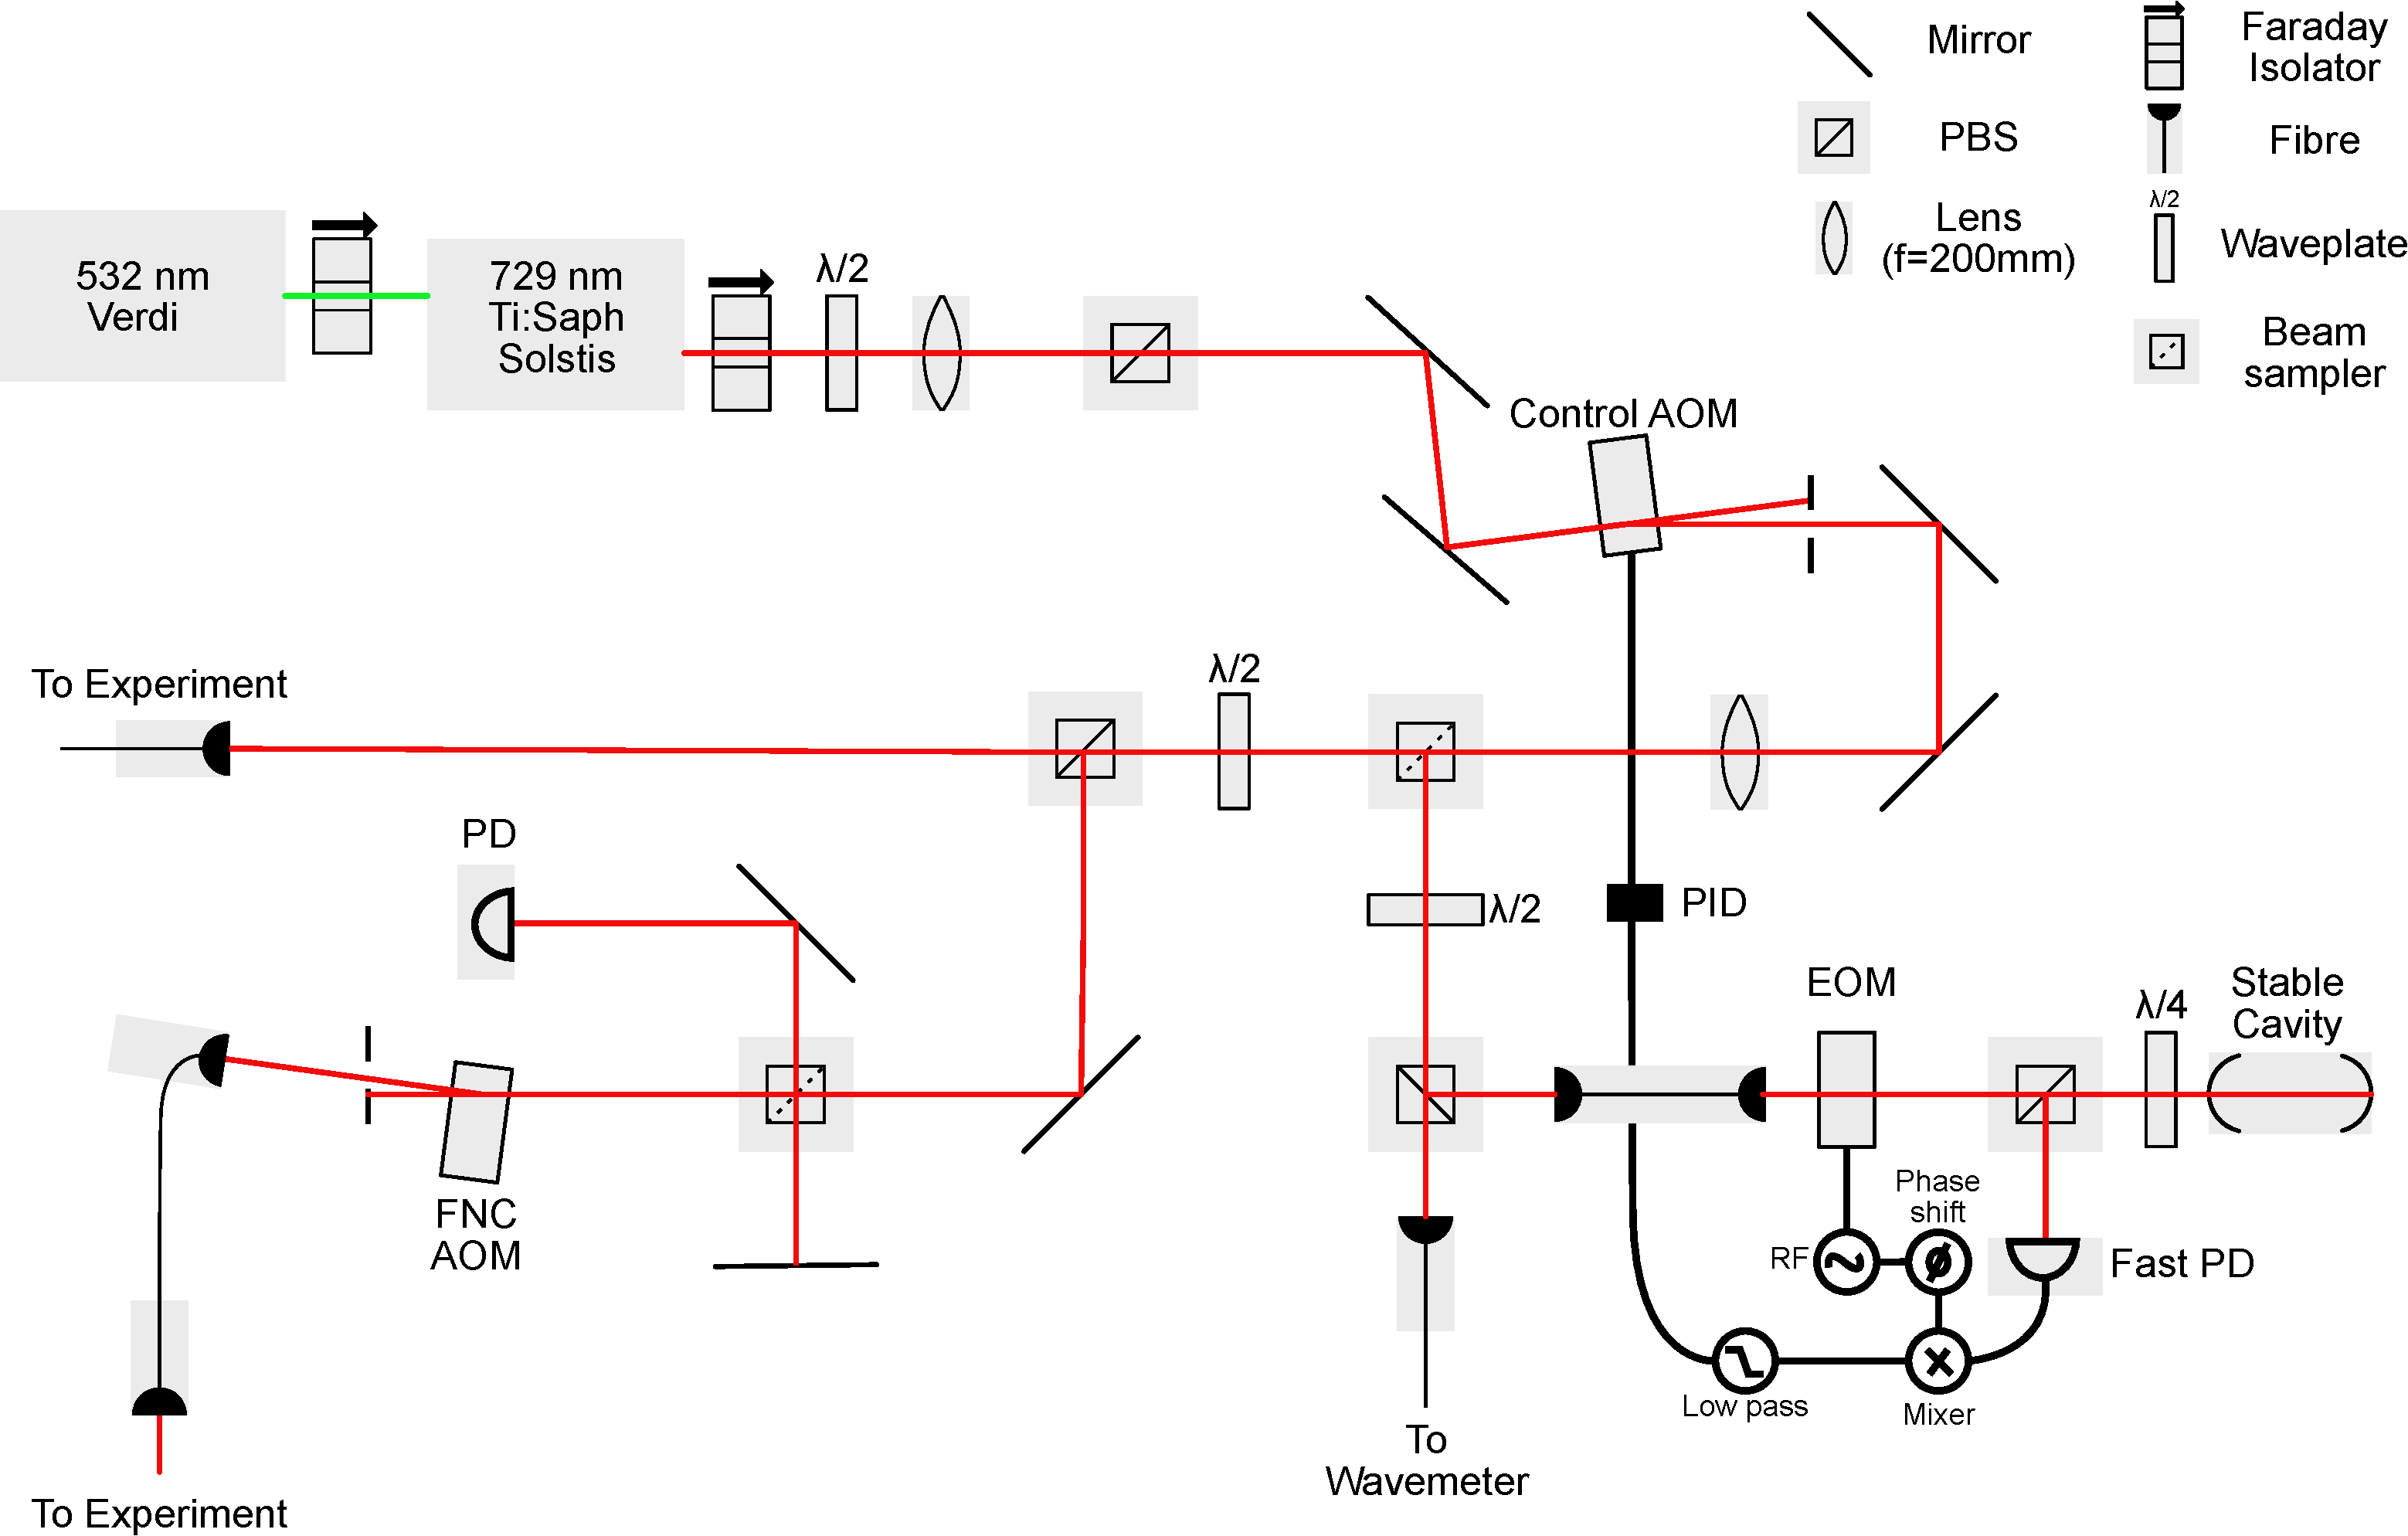
\includegraphics[width=\linewidth]{figures/729_path_small.pdf}
  \end{center}
  \caption{729 nm system}
  \label{fig:can}
\end{figure}

729 nm - Coherent control: As shown in figure X we will use the levels
4S\textsubscript{1/2} to 3D\textsubscript{5/2} with a 729 nm
quadrupole transition to define our qubit. Therefore the 729 nm laser
is used to implement single and multiqubit gates. We also use this
transition, after doppler cooling, for resolved sideband cooling to
step down to near the motional ground state of the ion crystal.

The natural lifetime of the metastable
3D\textsubscript{5/2} is around 1.1 s XrefBarton, giving a favorable
fundamental limit of coherence time for our chosen qubit.
%% i.e. the transition from D to S is dipole forbidden as they are the
%% same parity DelL != +-1.
This natural lifetime leads to a narrow 4S\textsubscript{1/2} to
3D\textsubscript{5/2} transition linewidth $\Gamma < 1$~Hz, and so
demands the use of a narrow linewidth laser. Further, we require a
high light intensity at the ion to drive sideband transitions due to a low
Lamb-Dicke factor for 729 transition, $\eta \approx 0.05$.
Pumped Ti:Saph laser systems have been shown to be both relatively
high power and narrow linewidth, making them suitable for our
experiment.

We pump an M2 Solstis Ti:Saph with 15 W of 532 nm light from a Verdi
system to produce around 4W of 729 nm light.  A schematic of the 729
nm system being built is shown in figure X. The frequency is
stabilized by the Pound-Drever-Hall (PDH) technique with a high
finesse cavity. PDH locking requires taking the laser light and
applying two sidebands via an electro-optical modulator (EOM). This
phase modulated light is then directed onto a stable cavity and a
reflected signal is directed onto a fast photodetector. The reflection
from the cavity consists of the interference between the carrier and
the sidebands which have been respectively altered by the cavity
transfer function. The photodetector signal is mixed down with the
same oscillator signal as provided to the EOM but delayed by some
phase, and finally low pass filtered to produce a signal for use as
the error signal in the servo loop.  This error gives a measure for
how far the carrier frequency is from the stable cavity resonant
frequency and is used for feedback onto the control AOM situated after
the Solstis.

Some of the 729 nm light is picked off and sent to a wavemeter to
monitor the frequency however the majority is coupled to two output
fibres for our experiment and another within the group. We require
fibre noise cancellation as we transport the 729 light from a laser
lab to the trapping lab by a 10 m single mode polarization maintaining
fibre and must ensure no phase noise is introduced.


Trial of Verdi C unsuccesful so far not achieving stable lasing with
solstis.
Improvements over Blade:
- 729 more convenient Ti:Saph freq -> Higher power, low noise
- access parallel to radial mode, Blade is 45 deg -> High Lamb Dicke
factor
- 729 more convenient for putting in fibre -> low charging


393 and 432 - PI 
Two step photoionization for isotope selectivity.

397 - Doppler Cooling, Fluorescent readout
Dipole transition for Doppler cooling as want fast scattering. Also
want higher freq light for more momentum transfer.
Fluor read out so that |0> bright and |1> dark.

854 and 866 - Repumping as branching ratio from P to S and D. So
during cooling and readout we lose population to these levels.

All of the above systems are Toptica Diode lasers coupled to a cavity
for PDH locking.


\subsection{Inside the vacuum}

\begin{figure}
  \begin{center}
   \noindent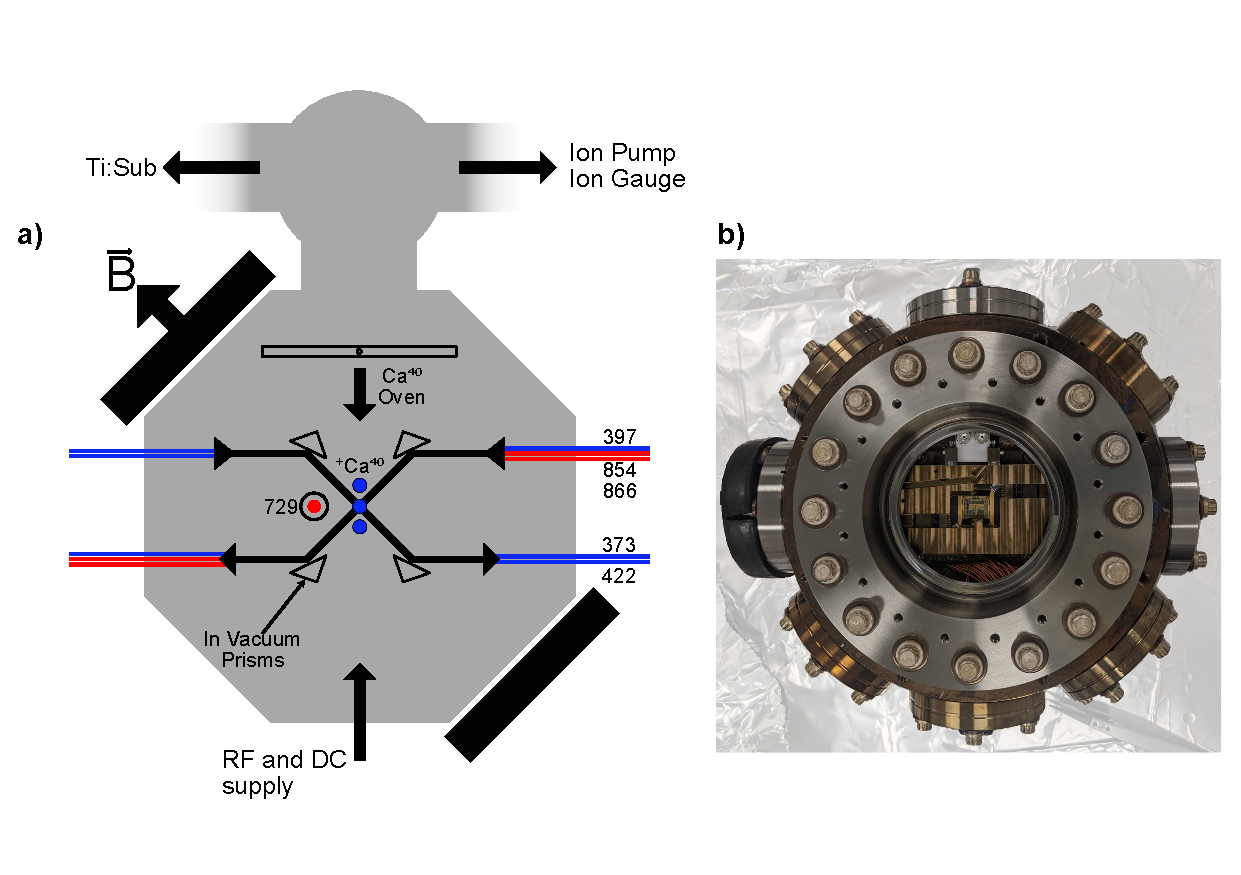
\includegraphics[width=\linewidth]{figures/vacuum_can.pdf}
  \end{center}
  \caption{Vacuum can}
  \label{fig:can}
\end{figure}

Here we shall describe the instrumentation required, and being
constructed, for decouping the ion from any unwanted external
environments. Our primary tools for this are working under Ultra High
Vacuum (UHV) and surrounding the vacuum system with electromagnetic
shielding. Inside the vacuum system we aim for a residual pressure of
less than $10^{-11}$ mbar. To reach this low a pressure, we must take
care in material choice and thoroughly clean and bake all material
within the vacuum system (a useful summary of tactics can be found in [ref]).

A schematic of the vacuum system can be seen in figure X. The system
consists of an octagonal experimental chamber connected to an Ion
pump, Ion Gauge and Ti:Sub pump. For optical access we have Dual CF100
viewports coated for 397 nm and 729 nm as well as two CF40 viewports
coated for 397 nm, 422 nm, 729 nm, 854 nm and 866 nm.

As discussed above, our ion will be located within a slit of the NPL
trap and so there is no visibility of the ions from the side CF40
viewports. We therefore are using in vacuum prisms to direct the light
onto the ions at XX degrees.

We use an electrical feedthrough on a CF40 flange to supply our trap
chip with both DC and RF voltages. As the DC cables run within close
proximity to the RF supply, electrical pick up is a potential issue
within our DC lines. We mitigate this through a low pass filter board
within close proximity of the trap chip. We implement a ``trap
stack'', seen in figure X, within the vacuum chamber consisting of the
trap chip, the outer chip carrier, an interposer, and the filter PCB.

\textsuperscript{+}Ca\textsubscript{40} was chosen for zero nuclear
spin and therefore simple energy level structure. However we now
cannot utilize hyperfine structure to find ``clock'' qubits which are
insensitive to magnetic field fluctuations and must instead remove
magnetic field noise from the environment. To suppress this noise 
we place the vacuum chamber within a box constructed from two layers
of 3mm thick MuMetal [ref]. The shielding was shown to suppress the
background field by a factor of 500 at its center.

\subsection{Single Addressing}

\begin{figure}
  \begin{center}
   \noindent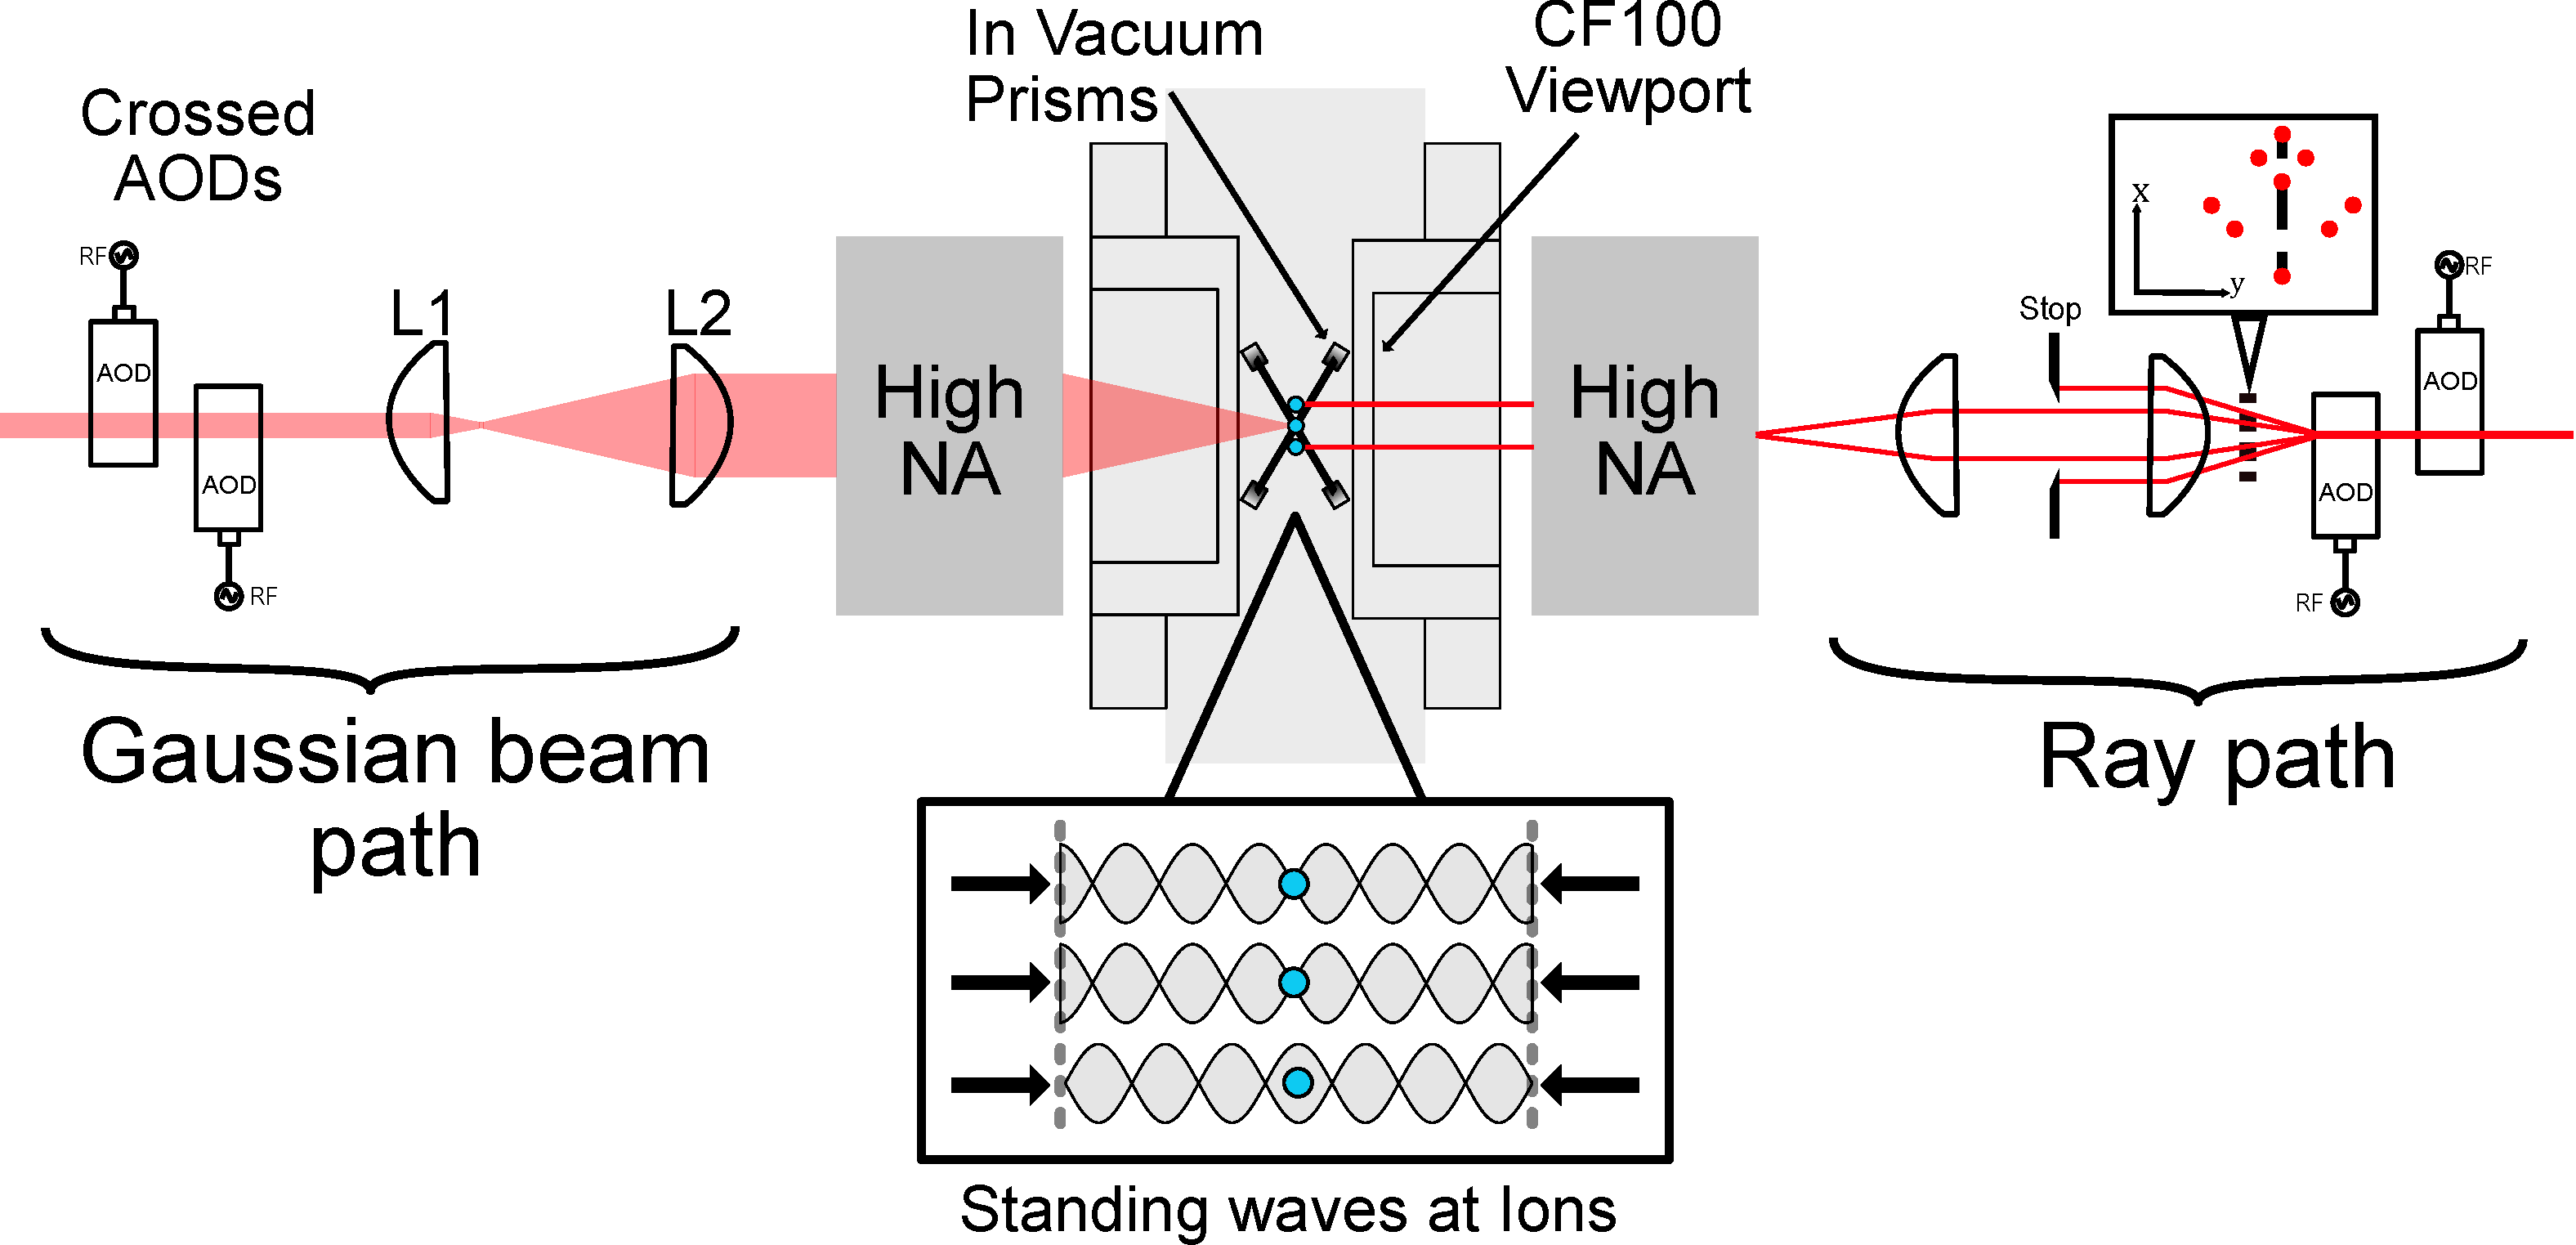
\includegraphics[width=\linewidth]{figures/vac_can_AOD_small.pdf}
  \end{center}
  \caption{Single addressing system}
  \label{fig:can}
\end{figure}

729 High NA (0.6) lens we can achieve waist radius of < 1 um.  With
our axial trap freq of XXX we get ion spacing of ~ 5um.  Using AOD
system we can traverse this ion chain.  Description of lens system
from AOD to ions.
Description on the mechanism on how AOD works (this is the same as an
AOM). Comparison between this and a fixed waveguide array. What
equations we need to find number of resolvable spots of the AOD
system. AOD have extra programmable control than waveguides which is
excellent as we are in an exploratory regime where we may want to
alter ion spacing/Dont want to use quartic potentials to make ions
evenly spaced.
We will use a crossed AOD design so that we have no overall frequency
shift as we scan along the ion chain.
Compact design to fit beam path within MuMetal box.
We want to create single addressing standing wave so must consider
stabilization technique from AOD. 
There is minimal path length differece compared to waveguide which is
ideal as we can stabilise at some central frequency and should be
stable at all ion locations.
Quick calculation to look at path length diff in wavlengths between
two extrema points on the ion chain. Note that this will give some
fixed relationship between the two beams if we assume that the small
seperation of beams paths is negligible (air density and current in
close proximity should be related).
Using two RF freq so that we can address two ions at the same
time. Initially looking at this we see that supplying two freqs and
amplifying we dont have crazy cross term amplitudes.
However addressing multiple ions at the same time comes at the cost of
photon freq cross terms i.e. spots that we dont want that are off
plane to our ions. This has two bad effects: Can get crosstalk to
other ions on the chain and lose power in our 729 system. First effect
we can mitigate by putting AOD at a > 45 deg angle (60 deg?) this
pushes the unwanted spots further from the chain. (sep to ion is
sqrt2/2 when at 45 deg). There is no easy way to mitigate the power
loss as two freq photons are barely distinguishable (maybe look again
at the two wavelength design aods). So this may limit us to only
addressing 2 or three ions at a time and using a global addressing
system through the prisms if all ions need to be addressed. Quick
power calculation though means we still have XXmW at each ion with an
intensity of XX which could drive CNulled gates at a speed of X.

%% Assuming our trapping potential to be quadratic, we have a spin system
%% coupled to a spring. The Jaynes Cummings Hamiltonian,
%% $$ H = H_{spin} + H_{HO} + H_{Int}, $$
%% summarises this coupled system.

subtitle FastGates Apparatus\\
*This has been (to be) incorportated into the above section. \\

Here we describe the design of the new ``FastGates'' system which is
tailored for the exploration of fast, non-adiabatic entangling
gates. Figure X shows a schematic of the vacuum can of ``FastGates''
with the addressing directions and magnetic field highlighted. Ca40
was chosen for initial experiments due to its simple energy level
structure, figure X, without hyperfine levels and with the option for
a quadrupole qubit between the S and D levels. An external magnetic
field of 5G is applied to define our Zeeman sublevels, this low field
will not allow state selective addressing by frequency, however allows
for polarization selective addressing. *** Check if 729 will actually
have linewidth for frequency addressing? *** The isotope having 0
nuclear spin and hence no hyperfine levels greatly simplifies control
schemes however precludes the option of using magnetically insensitive
``clock'' qubits. To ensure we do not greatly limit coherence time of
our quadrupole transition we use a MuMetal enclosure to suppress stray
environmental magnetic fields.


%}}}

%Outlook {{{
\section{Outlook}
    Current state of building up apparatus.
    Immediate next steps.
    Proposed first experiments?
    GANNT diagram?

%}}}
  
\end{document}
